\documentclass[times, 10pt,twocolumn]{article}
\usepackage{latex8}
\usepackage{times}
\usepackage{amssymb,amsthm,amscd,bm}
\usepackage{graphicx}

\usepackage[tight,footnotesize]{subfigure}

\usepackage{url}

\usepackage{listings}
\lstset{language=C++, basicstyle=\normalsize}

% take the % away on next line to produce the final camera-ready version
%\pagestyle{empty}

\newtheorem{rulez}{Rule}

\newcommand{\offset}{\textit{offset}}
\newcommand{\vtable}{\textit{vtable}}
\newcommand{\positive}{\textit{positive}}
\newcommand{\sequence}{\textit{sequence}}

\renewcommand{\~}{{\raise.35ex\hbox{$\scriptstyle\sim$}}}

\renewenvironment{itemize}{
    \begin{list}{\labelitemi}{\itemsep=-\parsep}
}{
	\end{list}
}

\newcounter{xcounter}
\renewenvironment{enumerate}{
    \begin{list}{\arabic{xcounter})}{\usecounter{xcounter} \itemsep=-\parsep}
}{
	\end{list}
}



\begin{document}

\title{Reconstruction of C++-specific constructs for decompilation}

\author{
A. Fokin\\
Moscow State University\\
Computational Math. and Cybernetics Dept.\\
Leninskie Gory, Moscow, Russia\\
apfokin@gmail.com
\and
Y. Derevenets\\
Institute for System Programming\\
Russian Academy of Sciences\\
25, Alexander Solzhenitsyn st., Moscow, Russia\\
yegord@ispras.ru\\
\and
K. Troshina\\
Institute for System Programming\\
Russian Academy of Sciences\\
25, Alexander Solzhenitsyn st., Moscow, Russia\\
katerina@ispras.ru
\and
A. Chernov\\
Moscow State University\\
Computational Math. and Cybernetics Dept.\\
Leninskie Gory, Moscow, Russia\\
cher@unicorn.cmc.msu.ru
}

\maketitle
%\thispagestyle{empty}

\begin{abstract}
This paper presents several methods useful for decompilation of C++ programs.
These methods allow automatic reconstruction of polymorphic class hierarchies
and exception raising and handling statements.

For reconstruction of polymorphic class hierarchies a new method
that does not use run-time type information is presented.
It relies only upon the way virtual table pointers are laid out inside objects
and is therefore compiler-independent to a large degree.

Depending on the application binary interface used by the compiler,
exception handling statements are located in the code using
data flow analysis and analysis of static exception handling structures.

A tool for automatic reconstruction of polymorphic class hierarchies
and exception raising and handling statements that implements the described techniques is presented.
This tool is implemented as a plugin for IDA Pro Interactive Disassembler.
Experimental study of the tool performance is provided.
\end{abstract}


\quad
\section{Introduction}
In this work we present several methods useful for decompilation
of C++ programs. These methods allow automatic reconstruction
of polymorphic class hierarchies and exception raising and
handling statements.
We presume
that no modifications of the assembly code were performed
after compilation (such as assembly-level obfuscation).
The problem of obtaining assembly code from an executable file
lies outside of the scope of this work.

For reconstruction of polymorphic class hierarchies we presume
that the program was compiled without RTTI (run-time type
information), as the opposite case is already well-studied \cite{fokin10, sabanal07, skochinsky06c}.
Besides, RTTI is considered to be frequently misused
\cite{stroustrup93}, and some modern applications written
in C++ refrain from using it.

An approach based on the analysis of vtables (virtual function tables),
constructors and destructors is used for reconstruction of
polymorphic class hierarchies. First, vtables are identified in the assembly.
Then the functions that work with pointers to vtables
are analyzed and classified as either constructors or destructors.
At the same time, inheritance relation on a set of vtables is reconstructed.
Correspondence between vtables and actual
classes is reconstructed via analysis of constructors.
Obtained information is then used for inference of the inheritance
relation on a set of classes.

%Virtual inheritance is not handled.
%In this case we also presume that virtual inheritance is not used.
%Virtual inheritance is not handled (virtual
%inheritance and inheritance utilizing virtual functions are
%two distinct C++ concepts, see \cite{stroustrup97} for details).

The presented method relies only upon the way vtable pointers are laid out
inside objects. Since this part of C++ ABI (application binary interface)
is implemented in the same way by most modern compilers, the presented method is
compiler-independent to a large degree.

As the implementation of the exception handling mechanism may differ greatly
depending on the ABI used by a compiler, several ABIs are considered.
Data flow analysis is used for identifying exception handling
statements in binaries compiled with Microsoft Visual C++ compiler.
After static exception handling structures are parsed, \lstinline{try} and
\lstinline{catch} block boundaries are reconstructed.
GCC on x86 and x64 architectures uses Dwarf2
table-based unwinding mechanism by default. Static exception handling
data used by Dwarf2 can be easily located and parsed. Additional
analysis then allows to reconstruct the boundaries of \lstinline{try} and \lstinline{catch} blocks.

The presented methods were implemented in a plugin for IDA Pro
interactive disassembler \cite{ida} and were tested on a variety
of open-source C++ software. We used MSVC 10.0 and g++ 4.4
for experimental study, but the tool also works for
other versions of these compilers provided they use the same C++ ABI.

This paper is organized as follows. Section
\ref{sectionRelatedWork} discusses related work.
A new method for class hierarchy reconstruction is presented in
Section \ref{sectionClasses}.
Section \ref{sectionExceptions} presents methods for reconstruction
of exception raising and handling statements.
Experimental results are discussed in Section \ref{sectionExperiments}.
Our conclusions and directions for future work are
presented in the last section.




\quad
\section{Related work}\label{sectionRelatedWork}
There are a lot of important works on decompilation.
In our opinion,
the following works are the closest to the topic of this paper.

Skochinsky \cite{skochinsky06e, skochinsky06c} has given a detailed description
of RTTI and exception handling structures used by MSVC,
along with the implementation details of some of the C++ concepts,
such as constructors and destructors.
He has presented several tools, which were implemented as scripts for
IDA Pro interactive disassembler. The first tool performs automatic analysis
of RTTI structures and can be used for reconstruction of polymorphic class hierarchies.
The second tool is used for automatic recognition of exception handling
statements in the assembly code. It does not reconstruct the boundaries of \lstinline{try} blocks.
These tools are based on pattern matching and do not always provide correct
results and cannot be used with compilers other than MSVC.

Kocchar \cite{kocchar02} has also examined details of the exception
handling mechanism used in MSVC. He has developed his own exception handling
library that replaces the default one.

Sabanal and Yason \cite{sabanal07} along with RTTI-based approach
to class hierarchy reconstruction
have proposed a technique based on the analysis of vtables and
constructors that can be applied even when RTTI structures are
not present in the assembly.
Constructors are identified by searching for \textbf{operator new}
calls followed by a function call.
Vtable analysis is used for polymorphic class identification.
Class relationship inference is done via analysis of constructors.
Authors have also presented several examples of successful class
hierarchy reconstruction.
However, several cases in which presented techniques may fail are
not considered.
These cases include \textbf{operator new} overloading,
constructor inlining and elimination of vtable references in
constructors due to optimizations.
The presented techniques also heavily rely on the usage of
MSVC-specific \textbf{\_\_thiscall} calling convention.

In \cite{fokin10} authors have proposed a
method for automatic reconstruction of class hierarchies
that does not rely on RTTI and performs well in cases
when aggressive optimizations are used by the compiler.
In this work we present a modification of this method
that performs much faster while offering comparable
error rates.




\quad
\section{Class hierarchy reconstruction}\label{sectionClasses}
For the reconstruction of polymorphic class hierarchies, vtables
are located first as described in \cite{fokin10}.

For two vtables $B$ and $D$, we say that vtable $B$ is a direct base of vtable $D$ if
one of the classes corresponding to vtable $B$ is a direct base of one of
the classes corresponding to vtable $D$.
Simple inheritance for vtables can then be defined as a transitive
closure of direct inheritance. The fact that vtable $D$ inherits
from vtable $B$ is denoted as $D \rhd B$ and is also referred to as
``$B$ is a base of $D$'' and ``$D$ is a child of $B$''. For example, for the
hierarchy on Fig. \ref{fig:abc} the following is true: 
$C \rhd A$, $C \rhd B$ and $B \rhd A$.

\begin{figure}[tb!]
\centering
  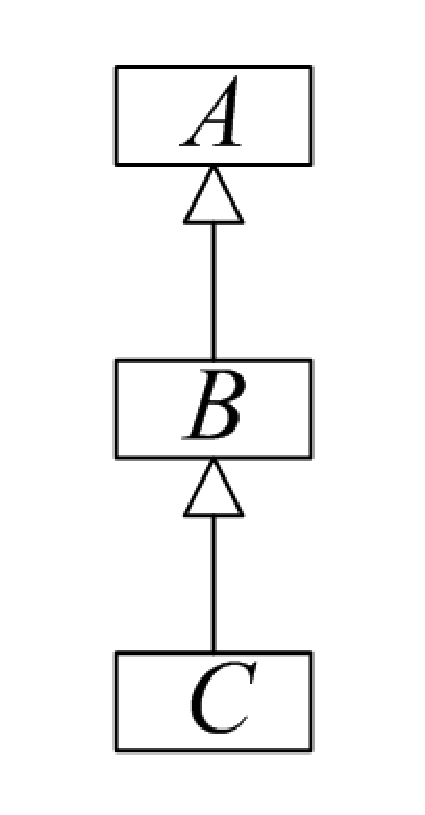
\includegraphics[height=3.0cm]{images/abc}
\caption{Example of a class hierarchy.}
\label{fig:abc}
\end{figure}

Class hierarchy reconstruction is performed via analysis of constructors
and destructors. Constructor of a class performs the following sequence
of operations \cite{cpp03, gray94}:
\begin{enumerate}
\item calls constructors of direct base classes;
\item calls constructors of data members;
\item initializes vtable pointer field(s) and
      performs user-specified initialization code in the body
      of the constructor.
\end{enumerate}

Conversely, a destructor deinitializes the object
in the exact reverse order to how it was initialized:
\begin{enumerate}
\item initializes vtable pointer field(s) and
    performs user-specified destruction code in the body of the destructor;
\item calls destructors of data members;
\item calls destructors of direct bases.
\end{enumerate}

Note that if multiple inheritance is used, a class may have
several vtable pointer fields, one for each polymorphic base.
In case of a ``deep'' inheritance hierarchy,
construction and destruction of an object may require many
successive initializations of vtable pointer field(s).
Experiments have shown that neither GCC nor MSVC optimize away
the last assignment in a non-inlined destructor.
% except for some special cases / inlining
That means that non-inlined destructor of an object always overwrites each
vtable pointer field with a pointer to the corresponding ``most-base'' vtable.




\quad
\subsection{Localization of constructors and destructors}\label{chapterLocalization}
Each vtable is referenced only from constructors and destructors
of the corresponding class~--- its address is written into
vtable pointer field of the object being constructed or destructed.

Constructors and destructors can be inlined, so there
can be several constructor and destructor calls inside a single
assembly subroutine.
To address this problem, an interprocedural data flow analysis as described
in \cite{aho06} is used. 
It is employed to detect code sites where one or more memory locations that
differ from each other by a constant offset are overwritten with
pointers to vtables.
These code sites are referred to as \textit{vtable access sites}.
Each vtable access site is either a constructor or a destructor
and is uniquely identified with a set of addresses
of the instructions that initialize vtable pointer field(s).
Inclusion of vtable access sites is defined in terms of
inclusion of these address sets.

\begin{figure}[tb!]
\centering
  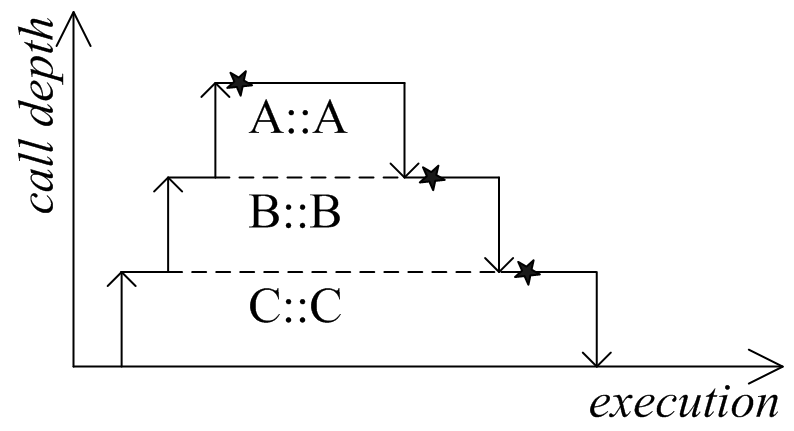
\includegraphics[width=7.0cm]{images/ctor}
\caption{Outline of constructor execution for class \lstinline{C} from Fig \ref{fig:abc}.
Initializations of vtable pointer field are marked with $\bigstar$.}
\label{fig:ctor}
\end{figure}

Note that vtable access sites are likely to span several subroutines. In this
case several vtable access sites are created: one for the
enclosing subroutine and one for the nested subroutine, the former including the latter.
It is performed this way because vtable access site in a nested
subroutine clearly corresponds to a different constructor or destructor than the one
in the enclosing subroutine, 
and the bigger the number of recognized constructors and destructors, the easier class
hierarchy reconstruction.

\begin{figure}[tb!]
\centering
  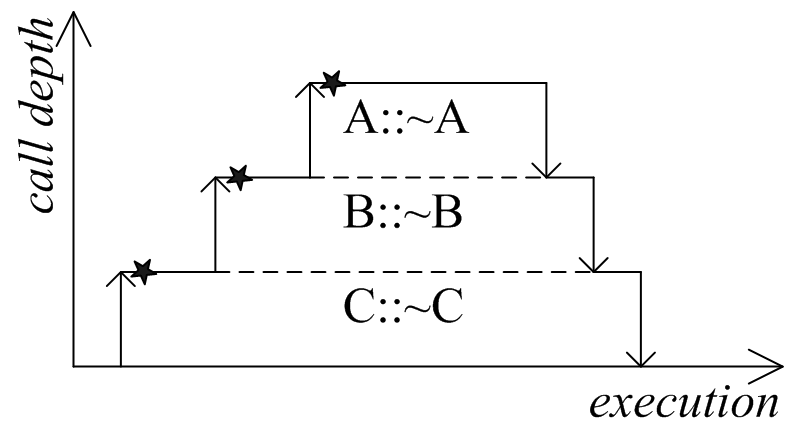
\includegraphics[width=7.0cm]{images/dtor}
\caption{Outline of destructor execution for class  \lstinline{C} from Fig \ref{fig:abc}.
Initializations of vtable pointer field are marked with $\bigstar$.}
\label{fig:dtor}
\end{figure}

Consider an example on Fig. \ref{fig:dtor}.
As can be seen, vtable access site for \lstinline{C::~C} includes vtable
access site for \lstinline{B::~B} because \lstinline{C::~C} calls
\lstinline{B::~B} for \lstinline{this} object.

Every vtable access site is associated with
a set of pairs (\positive\,\offset, \vtable\,\sequence).
Vtables are stored in \vtable\,\sequence~in an order in which their addresses
are written at the corresponding \positive\,\offset.

Consider an example on Fig. \ref{fig:dtor}.
Analysis of destructor for class \lstinline{C} will generate three vtable access sites
with the following sets of pairs associated with them:
$\{(0, (C, B, A))\}$ (for \lstinline{C::~C}),
$\{(0, (B, A))\}$ (for \lstinline{B::~B}),
$\{(0, (A))\}$ (for \lstinline{A::~A}).




\quad
\subsection{Vtable inheritance reconstruction}
First we consider a case where multiple inheritance is not used.
In this case each vtable access site is associated with only
one pair (\positive\,\offset, \vtable\,\sequence).

The order in which vtable pointer field initializations are performed
is determined by the inheritance order. Consider a hierarchy
on Fig. \ref{fig:abc}.
Outlines of constructor and destructor execution for class
\lstinline{C} are provided on Fig. \ref{fig:ctor} and \ref{fig:dtor}
correspondingly. As can be seen, in a call to constructor vtable
pointer field is overwritten in a ``base-to-derived'' order,
while in a call to destructor it is overwritten in a
``derived-to-base'' order.

Since each vtable access site corresponds to either a constructor
or a destructor, the inheritance direction in a \vtable\,\sequence~is
either ``base-to-derived'' (for constructors) or ``derived-to-base'' (for destructors).
For example, consider a vtable access site for \lstinline{C::C} with an associated pair
$(0, (A, B, C))$ (see Fig. \ref{fig:ctor}). It is a constructor, therefore
the inheritance direction in $(A, B, C)$ is ``base-to-derived'',
i.e. $A \lhd B \lhd C$. This matches the actual
inheritance direction (Fig. \ref{fig:abc}). Therefore, the following rule
can be applied.

\begin{rulez}
If \textit{vtable access site} is associated with a pair $(\offset, (A_1, \ldots, A_n))$,
then either $A_1 \lhd \ldots \lhd A_n$ or $A_1 \rhd \ldots \rhd A_n$.
\end{rulez}

As can be seen on Fig. \ref{fig:ctor} and \ref{fig:dtor},
in a call to a constructor, vtable pointer field is initialized \textbf{after} a
call to the constructor of the base class, while in a call to a destructor,
vtable pointer field is initialized \textbf{before} a call to the destructor of
the base class. Therefore each vtable access site that spans
several assembly subroutines can be identified as either a constructor or
a destructor using the following rule.

\begin{rulez}
Let some vtable access site span several assembly subroutines. If the initialization of
vtable pointer field precedes the call to the nested subroutine that also initializes that field,
then this vtable access site is a destructor. Otherwise,
it is a constructor.
\end{rulez}

It can happen that all nested constructor or destructor calls were inlined.
In this case all initializations of vtable pointer field of
vtable access site are located in one assembly subroutine and this rule cannot be applied.
Instead, the following rules are used.

\begin{rulez}
If one vtable access site contains the other one, then either both of them are
constructors, or both of them are destructors.
\end{rulez}

As it was denoted in Section \ref{chapterLocalization}, vtable access site
inclusion is defined in terms of inclusion of associated sets of addresses
of instructions that initialize vtable pointer field(s).
Rule 3 is a direct consequence of the fact that a constructor cannot call
a destructor for \lstinline{this} object, as well as a destructor cannot
call a constructor for \lstinline{this} object.

\begin{rulez}
If vtable access site is associated with a pair
$(\offset, (A_1, \ldots, A_{k_1}, \ldots, A_{k_2}, \ldots, A_n))$, and the size of vtable
$A_{k_1}$ is less then the size of vtable $A_{k_2}$, then $A_1 \lhd \ldots \lhd A_n$.
\end{rulez}

According to the C++ inheritance rules \cite{cpp03},
if there are more virtual functions in vtable $A_{k_2}$ than in vtable $A_{k_1}$,
then $A_{k_2}$ cannot be a base of $A_{k_1}$. Rule 2 is a direct consequence of this fact
applied to Rule 1.

\begin{rulez}
If a vtable access site is associated with a pair
$(\offset, (A_1, \ldots, A_{k_1}, \ldots, A_{k_2}, \ldots, A_n))$, and $i$-th virtual function
in vtable $A_{k_1}$ is pure and $i$-th virtual function in vtable $A_{k_2}$ is not,
then $A_1 \lhd \ldots \lhd A_n$.
\end{rulez}

This rule is a direct consequence of Rule 1 and the fact that in C++ it is impossible to
override a virtual function that is not pure with a pure one \cite{cpp03}.

Application of each of the Rules 1-5 gives an inheritance
relation on vtables in the corresponding vtable sequence.
Thus, by applying Rules 1-5 to vtable access sites,
inheritance relation on a set of vtables is reconstructed.

Obviously, there may be cases when these rules won't
be sufficient to completely reconstruct inheritance
relation on a set of vtables. However, as it is shown
in Section \ref{sectionExperiments}, in practice
such cases are nearly nonexistent.

If multiple inheritance is used, then almost the same rules can be applied.
The only difference is that instead of one
(\positive\,\offset, \vtable\,\sequence) pair
each vtable access site will have several.
Modified rules for multiple inheritance are not
presented here as they can be easily derived
from the ones for single inheritance.




\quad
\subsection{Polymorphic class hierarchy reconstruction}\label{chapterReconstruction}
Constructors and destructors for ``most-base'' classes
overwrite vtable pointer field only once, and therefore
cannot be easily differentiated if not nested into some other
constructor or destructor. That's why in this case they are
classified as constructors.

Classes are reconstructed via analysis of vtable
access sites that are constructors. Classes
are uniquely identified with a set of
(\offset, \vtable) pairs, \offset~being the
offset of \vtable~in this class.
This set of pairs can be constructed by
picking the last vtable from each of
vtable sequences associated with a class.

Generally speaking, the fact that vtable belongs to a class does not
necessarily mean that this class has inherited it.
However, inheritance and inclusion as a field are normally indistinguishable.
Besides, in most cases polymorphic classes are included by pointer.
That's why by default it is presumed that all vtables belonging to
a class were generated as a result of inheritance.

Constructors for ``most-base'' abstract classes
may have been optimized away by the compiler. That's why for each
vtable that has no parents,
a class containing it at offset 0 is constructed.

After a set of classes is constructed, inheritance relation inference
is performed as described in \cite{fokin10}. As a result, for
each polymorphic class in a program the following is reconstructed:
\begin{itemize}
\item vtables;
\item direct base classes;
\item offsets to the instances of direct base classes inside \lstinline{this} object;
\item constructors and destructors.
\end{itemize}




\quad
\section{Reconstruction of exception raising and handling statements}\label{sectionExceptions}
C++ standard defines semantics of exception raising and handling,
but leaves its implementation up to compiler vendors. The way exception handling is
implemented depends on the ABI used by the compiler.

Exception handling in C++
consists of the following steps:

\begin{enumerate}
\item throwing an exception;
\item stack unwinding;
\item execution of exception handler.
\end{enumerate}

All the information necessary to perform these steps must be present in the
assembly program.



\quad
\subsection{Exception handling in MSVC}
In MSVC C++ exception handling is implemented on top of OS-supplied Structured
Exception Handling (SEH) mechanism. For each thread a stack of
\lstinline{EXCEPTION_REGISTRATION} structures is maintained, with \textbf{fs:[0]} pointing to
the top of it. Each such structure contains a pointer to an exception handling routine.
When exception is raised, control is transferred to the kernel, which then calls the relevant
exception handling routine \cite{pietrek97}. Normally, \lstinline{EXCEPTION_REGISTRATION}
structure is allocated on the stack at the beginning of a function and \textbf{fs:[0]}
is modified to point to it.

For C++ exception handling extended \lstinline{EXCEPTION_REGISTRATION} structure is used \cite{skochinsky06e}.
{
\lstset{basicstyle=\small}
\begin{lstlisting}
struct EXCEPTION_REGISTRATION {
  /** Previous element in a stack. */
  EXCEPTION_REGISTRATION *prev;
  /** Exception handling routine. */
  void *handler;
  /** Current unwind state id. */
  int id;
  /** Saved ebp register. */
  DWORD ebp;
};
\end{lstlisting}
}

When an exception is thrown during execution of a function, destructors for
stack-allocated objects must be called. Unwind state field of
\lstinline{EXCEPTION_REGISTRATION} structure is an integer describing the set of
objects that must be destroyed when an exception is thrown. It is modified
every time an object is constructed or destructed and when execution enters
\lstinline{try} and \lstinline{catch} blocks.
Normally, when an object is constructed, unwind state is incremented by one,
and when it is destructed, it is decremented by one.

\begin{figure}[tb!]
\centering
  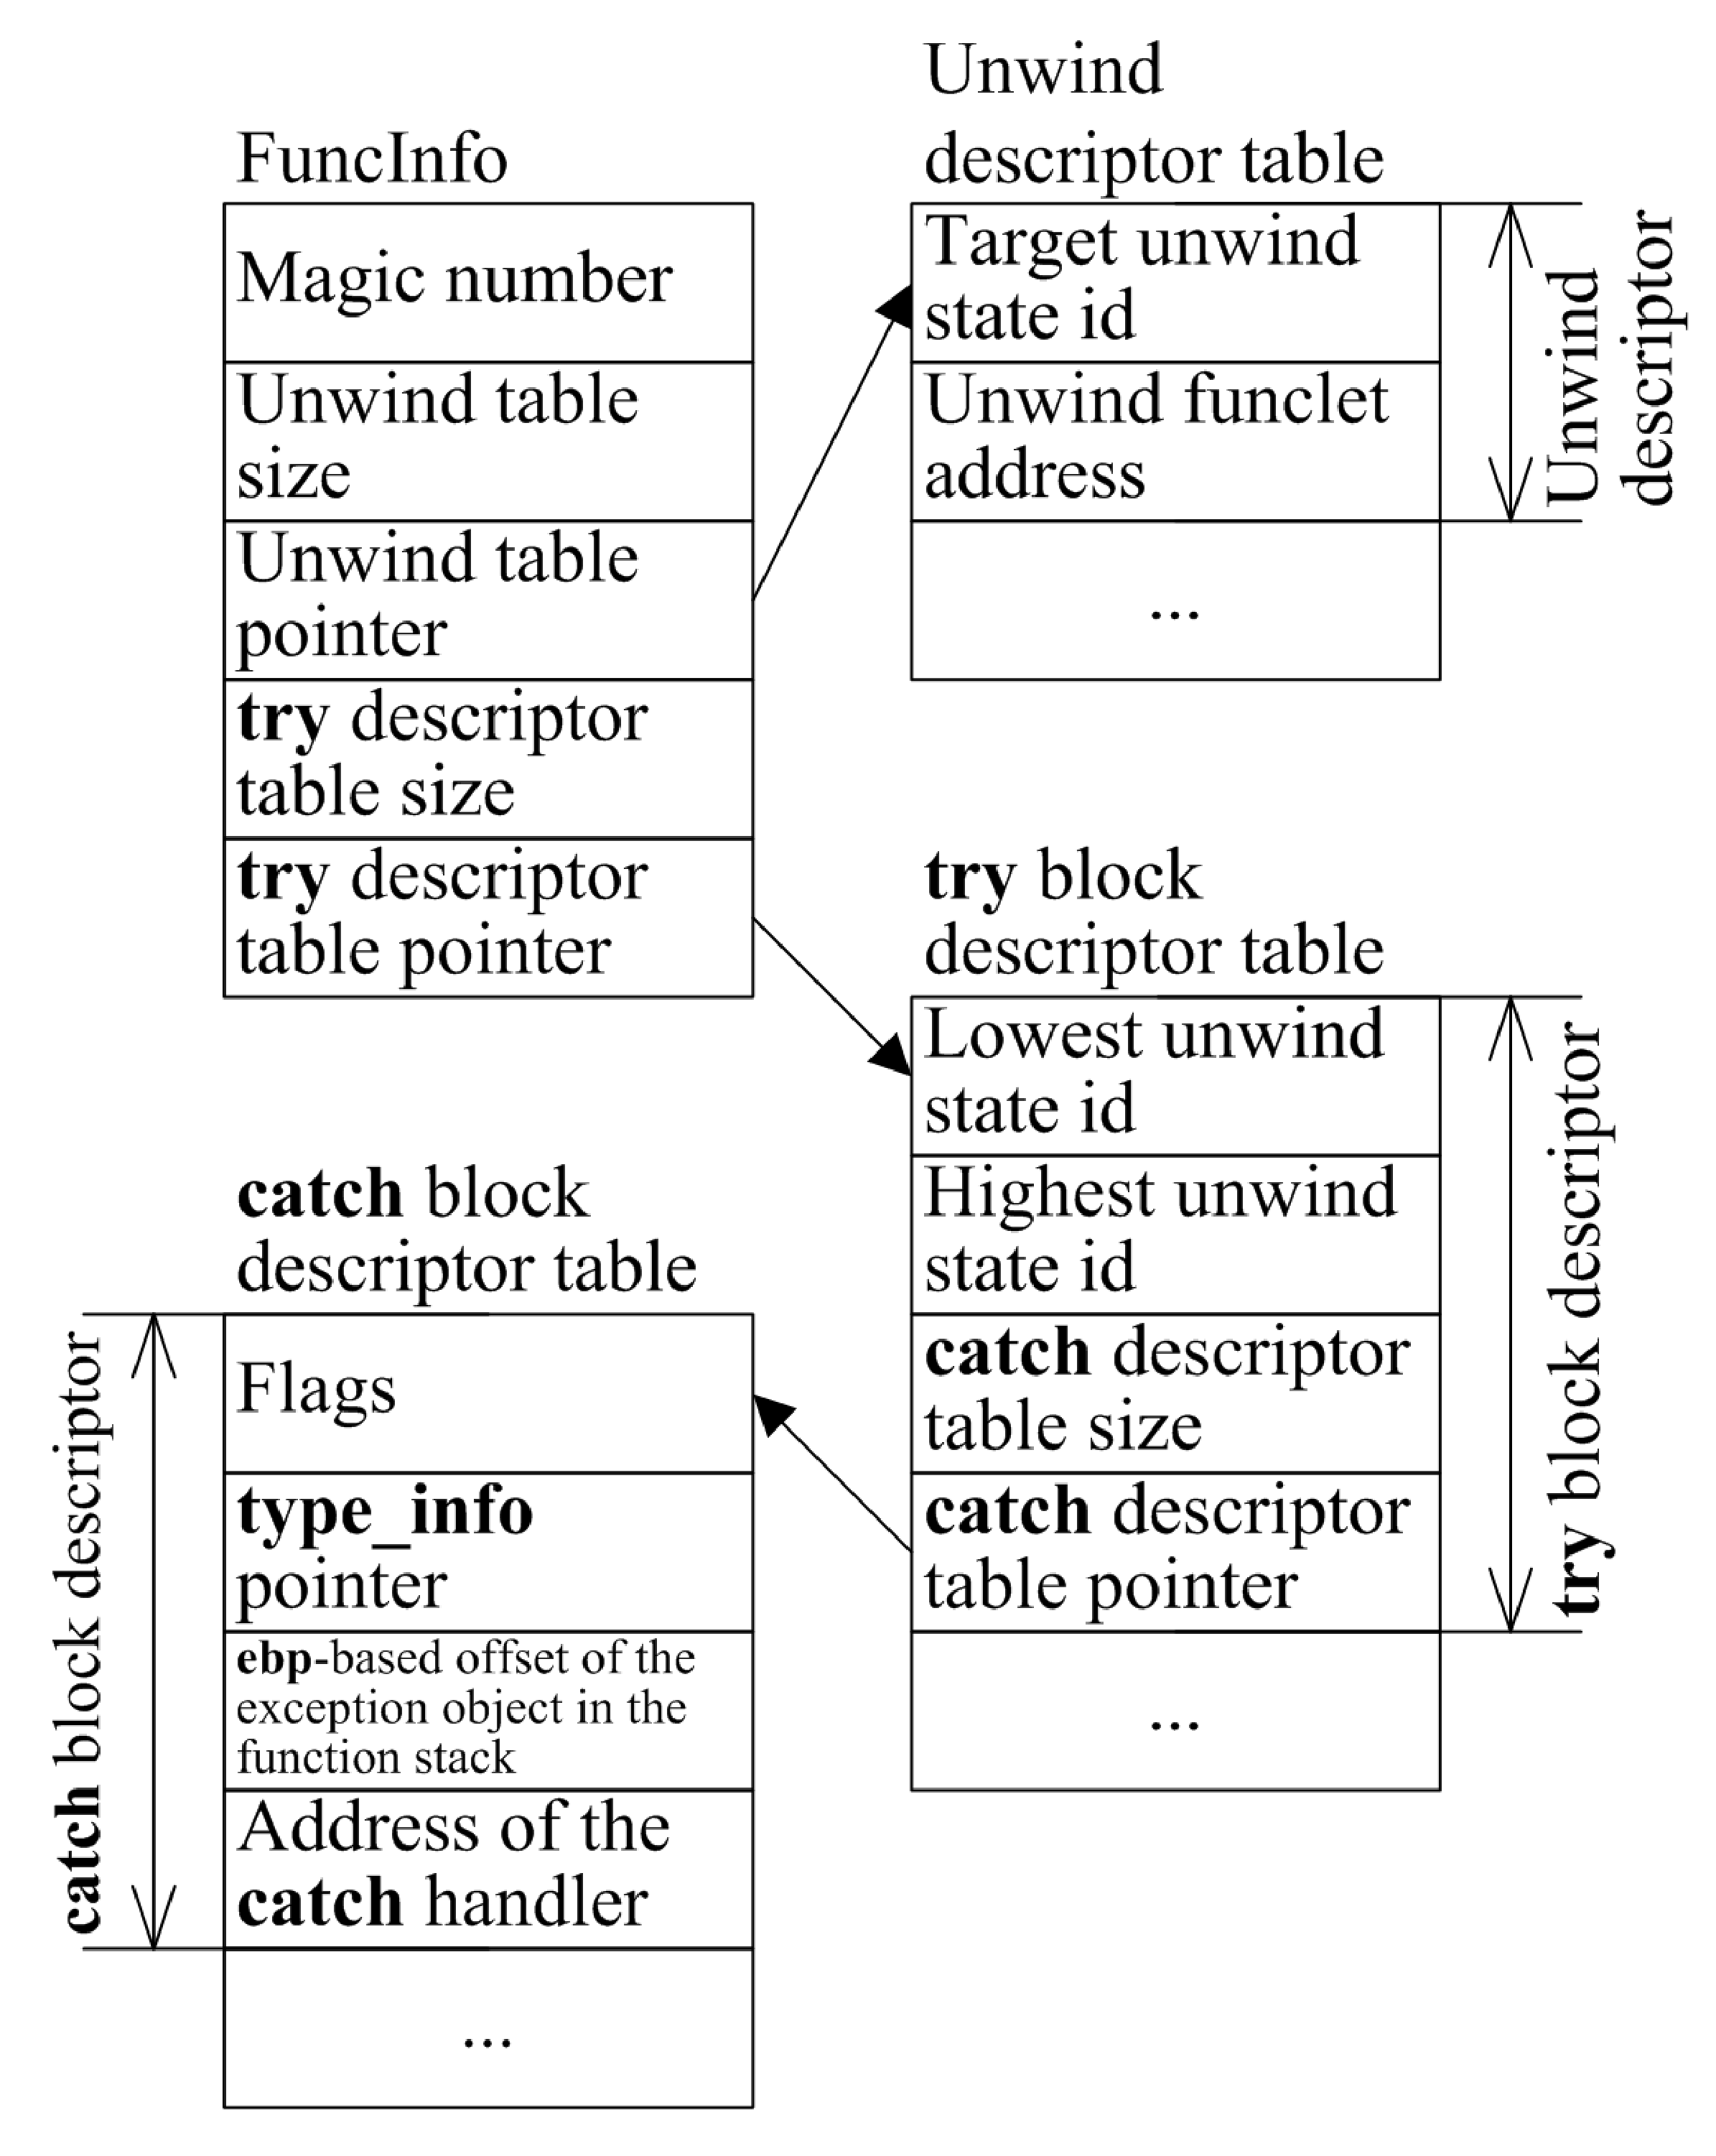
\includegraphics[width=8.0cm]{images/msvce}
\caption{Structures used by MSVC for exception handling.}
\label{fig:msvce}
\end{figure}

For each function MSVC registers a SEH exception handler which ends with a call to
\lstinline{__CxxFrameHandler} function. This function takes a pointer to
FuncInfo structure in \textbf{eax} register. FuncInfo structure fully describes
all \lstinline{try} and \lstinline{catch} blocks and unwindable objects in a function 
(see Fig. \ref{fig:msvce}). 
This structure contains \cite{skochinsky06e}:
\begin{itemize}
\item pointer to the table of unwind descriptors. Elements of this table describe which destructors
    must be called for each unwind state;
\item pointer to the table of \lstinline{try} block descriptors.
\end{itemize}

In turn, each \lstinline{try} block descriptor contains the following information:
\begin{itemize}
\item the highest and the lowest unwind states inside the \lstinline{try} block;
\item pointer to the table of associated \lstinline{catch} block descriptors for 
    this \lstinline{try} block. 
    Each element in this table contains a pointer to the \lstinline{type_info} 
    of the exception class and a pointer to the catch handler.
\end{itemize}

Each catch handler returns the address where to resume execution, i.e. the position
just after the \lstinline{try} block.



\quad
\subsubsection{Reconstruction of exception handling statements}
To reconstruct \lstinline{try} and \lstinline{catch} blocks the following procedure is used:
\begin{itemize}
\item Locations in the program where \lstinline{EXCEPTION_REGISTRATION} structure is allocated
    on the stack are found. They are simple to detect via data flow analysis as the allocation
    of this structure involves copying of the value of \textbf{fs:[0]} to the stack
    (\lstinline{prev} field of \lstinline{EXCEPTION_REGISTRATION} structure is initialized with it).
\item Data flow analysis also makes it possible to find initial values of the other fields of
    \lstinline{EXCEPTION_REGISTRATION} structure, including the pointer to exception
    handling routine.
\item Data flow analysis of exception handling routine is performed to find the value of
    \textbf{eax} register before a call to \lstinline{__CxxFrameHandler} function. This value
    is a pointer to the statically allocated FuncInfo structure.
\item FuncInfo structure is parsed, thus giving the addresses of unwind and catch handlers.
\item Value of the \lstinline{id} field of \lstinline{EXCEPTION_REGISTRATION} structure
    at each point in the function is found via data flow analysis. \lstinline{try} block boundaries are
    then restored by inspecting the state range of \lstinline{try} block descriptor and the addresses returned by
    corresponding \lstinline{catch} handlers.
\end{itemize}



\quad
\subsubsection{Reconstruction of exception raising statements}
\lstinline{throw} statements are translated by the compiler into calls of
\lstinline{_CxxThrowException} function.
{
\lstset{basicstyle=\small}
\begin{lstlisting}
void _CxxThrowException(
  void *exception,
  ThrowInfo *throwInfo
);
\end{lstlisting}
}

This function raises a SEH exception with custom parameters that include
pointers to the exception object and its \lstinline{ThrowInfo} structure
\cite{skochinsky06e}.
{
\lstset{basicstyle=\small}
\begin{lstlisting}
struct ThrowInfo {
  /** Const-volatile attributes. */
  DWORD attributes;
  /** Exception destructor. */
  void (*destructor)();
  /** Forward compatibility handler. */
  DWORD compat;
  /** List of types that can catch
   * this exception, i.e. the actual
   * type and all its ancestors. */
  CatchableTypeArray *catchableTypes;
};
\end{lstlisting}
}

If \lstinline{catch} block's parameter type is a base class and exception is its derived class, then this
\lstinline{catch} block should still be invoked. That's why \lstinline{CatchableTypeArray} contains
\lstinline{type_info} pointers for exception class and all its direct and indirect bases.
When checking whether \lstinline{catch} block can process the thrown exception, \lstinline{type_info}
of the \lstinline{catch} block's parameter is compared with all the \lstinline{type_info}'s available
through the \lstinline{ThrowInfo} structure. If any match is found then the \lstinline{catch} block is invoked.

To reconstruct \lstinline{throw} statements it is sufficient to locate the calls to
the \lstinline{_CxxThrowException} function in the code, find the values of its
parameters via data flow analysis, and parse the statically
allocated \lstinline{ThrowInfo} structure.




\quad
\subsection{Exception handling in GCC}
GCC under x86 and x64 architectures uses Dwarf2 table-based unwinding mechanism by default.
In Dwarf2 each function is associated with a set of \textit{call sites}. Call sites
are code sections that can potentially throw an exception, e.g. function calls or
\lstinline{throw} statements. Each call site is associated with a \textit{landing pad}.
Landing pad is a code block that calls destructors and transfers execution to the
corresponding \lstinline{catch} block. Information on call sites and landing pads is
statically allocated and is present in the assembly. Details on how exception
handling is performed using these structures is given in \cite{gccabi}.

\begin{figure}[tb!]
\centering
  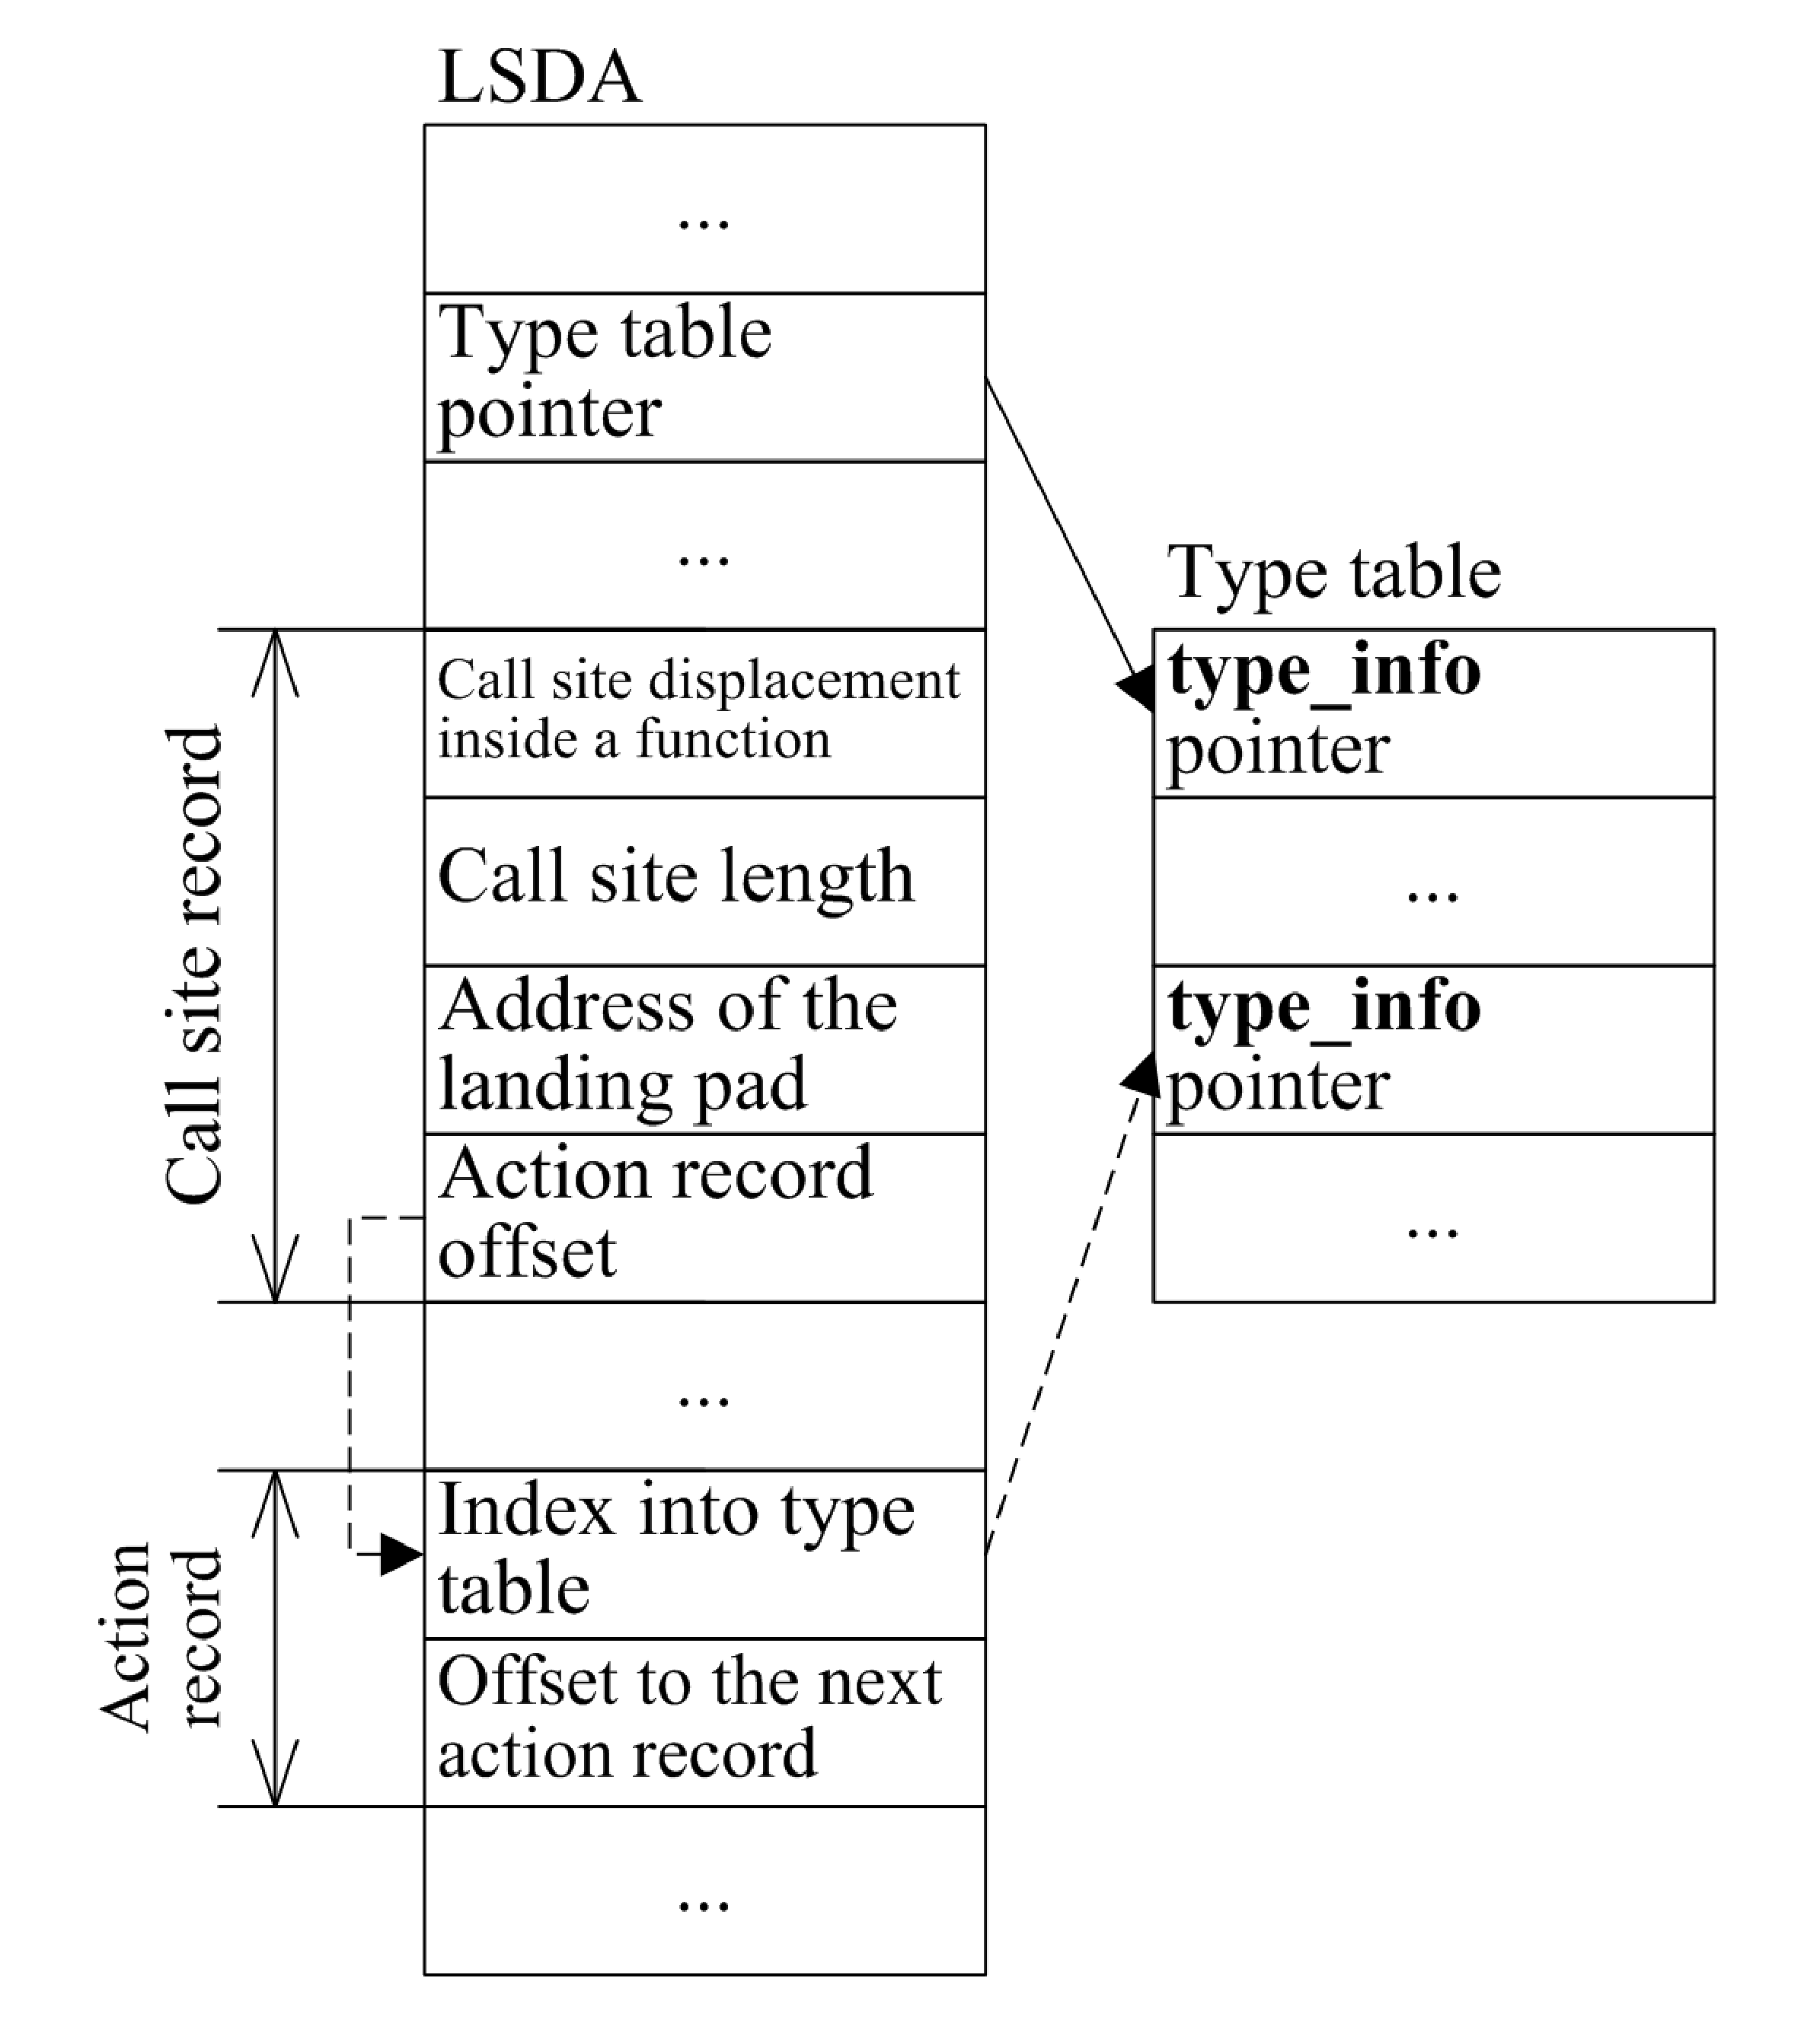
\includegraphics[width=8.0cm]{images/gcce}
\caption{Structures used by GCC for exception handling.}
\label{fig:gcce}
\end{figure}

\textbf{.eh\_frame} section of the assembly contains information on stack frames
that is needed for stack unwinding. Its format is described in \cite{linuxspec}.
Frame descriptor for each function contains a pointer to the
Language Specific Data Area (LSDA) containing exception handling information (see Fig. \ref{fig:gcce}).
LSDAs are stored in \textbf{.gcc\_except\_table}
section.

For each call site LSDA contains:
\begin{itemize}
\item call site displacement inside a function;
\item call site length;
\item address of the corresponding landing pad;
\item pointer to the list of \textit{action records}.
\end{itemize}

Each action record contains an index of an element in the type table, which
consists of pointers to \lstinline{type_info} structures.
List of action records in LSDA describes
exception types that can be handled by the landing pad.

Information stored in the statically allocated structures in
\textbf{.eh\_frame} and \textbf{.gcc\_except\_table} sections must be
parsed in order to reconstruct \lstinline{try} and \lstinline{catch}
blocks.
This presents no difficulties as the format of these structures
is documented.

Before the runtime transfers control to a landing pad, it 
finds the index of exception's \lstinline{type_info}
in the type table. This index is passed in \textbf{edx} register
to the landing pad. Dispatch to the \lstinline{catch} block body is
performed via a \lstinline{switch} on this index.

\begin{figure}[tb!]
\centering
{
\lstset{basicstyle=\small, language=[x86masm]Assembler}
\begin{lstlisting}
; Destructor calls skipped.
; Exception pointer is passed in eax.
mov [ebp - 24], eax
; Index in the type table is passed in edx.
mov [ebp - 28], edx
cmp [ebp - 28], 2
je catch_block_2
cmp [ebp - 28], 1
je catch_block_1
mov eax, [ebp - 24]
mov [esp], eax
call _Unwind_Resume
\end{lstlisting}
}
\caption{Example of a landing pad.}
\label{fig:lpad}
\end{figure}

Consider an example of the landing pad on Fig. \ref{fig:lpad}.
Since each \lstinline{catch} block starts with a call to \lstinline{__cxa_begin_catch}
and ends with a call to \lstinline{__cxa_end_catch},
\lstinline{catch} blocks can be reconstructed by examining
the landing pad and the locations it references.

Different destructors must be called when exception is thrown from
different call sites. That's why the compiler generates several landing
pads for each \lstinline{try} block.
However, the part of the landing pad that performs dispatch to
the \lstinline{catch} block (the part on Fig. \ref{fig:lpad}) is shared by all
landing pads for all call sites of a single \lstinline{try} block.

Therefore call sites belonging to the same \lstinline{try} block can be identified
by analyzing their corresponding landing pads~--- if two landing pads
share the same dispatch block, then their corresponding call sites
belong to the same \lstinline{try} block. Extents of the \lstinline{try}
block are then reconstructed by uniting all its corresponding
call sites.

Exception raising in GCC is performed via a call to the \lstinline{__cxa_throw} function.
{
\lstset{basicstyle=\small}
\begin{lstlisting}
void __cxa_throw(
  void *exception,
  type_info *typeInfo,
  void (*destructor)(void *)
);
\end{lstlisting}
}

To reconstruct throw statements it is sufficient to locate the calls
to \lstinline{__cxa_throw}, find the values of its parameters via
data flow analysis, and parse the statically allocated \lstinline{type_info}
structure.

Note that \lstinline{type_info} structure used by GCC provides
all the necessary information on the base classes \cite{gccabi}.
That's why there is no need to supply a list of \lstinline{type_info}
pointers for all the bases of exception class as it is in case of MSVC.






\quad
\section{Implementation and experimental results}\label{sectionExperiments}
The presented methods were implemented in a plugin
for IDA Pro interactive disassembler.
The plugin is available for download at \url{http://decompilation.info}.

The plugin was tested on a variety of open-source software written in C++.
The process used for testing class hierarchy reconstruction correctness is as follows.
First, the program is compiled with optimizations and RTTI, and
RTTI-aware class hierarchy reconstruction algorithm is used to collect information
on polymorphic class hierarchy. This algorithm always provides correct results \cite{fokin10}.
The program is then recompiled with optimizations and debug information but without RTTI.
Class hierarchy reconstruction algorithm described in Section \ref{sectionClasses} is applied,
and debug information is used to restore the correspondence between vtables and
actual polymorphic classes.
Results of the two class hierarchy reconstruction algorithms are then compared.

\begin{figure}[htb!]
\footnotesize
\begin{tabular}{| l | r | r | r | r |}
\hline
Application &         doxygen & shareaza & notepad++ & mysqld \\
\hline
Running time (old) &    7.9s  &   18.9s  & 0.7s      & n/a    \\
\hline
Running time &          3.2s  &   4.1s   & 0.6s      & 7.2s\\
\hline
Vtables found &         415   &   1128   &   95      & 950 \\
\hline
Non-vtables &           0\%   &   0\%    &   0\%     & 0.2\% \\
\hline
Vtable mismatches &     8.6\% &    4.1\% & 4.0\%     & 4.2\% \\
\hline
Classes found &         401   &   1108   &  95       & 974 \\
\hline
Non-classes &           0.9\% &    0.6\% &   0\%     & 3.4\% \\
\hline
Class mismatches &      9.7\% &    6.5\% & 10.5\%    & 8.0\% \\
\hline
\end{tabular}
\caption{Test results.}
\label{fig:tests}
\end{figure}

Test results
for doxygen (source code documentation generator),
notepad++ (text editor), shareaza (peer-to-peer file sharing client),
and mysqld (server daemon of MySQL relational database management system)
are presented on Fig. \ref{fig:tests}.
Tests were performed on an Intel Core 2 CPU running at 2.8Ghz.

``Running time (old)'' refer to the running time of the previous
version of the plugin
that was presented by the authors in \cite{fokin10}.
As can be seen, new method for class hierarchy reconstruction performs in our tests
up to five times faster.

For each of the analyzed applications all vtables present in
the assembly were found.
``Non-vtables'' refer to reconstructed vtables that were not present
in the source program. Static arrays of function pointers that are
used in the same way as vtables fall into this category.

``Non-classes'' refer to reconstructed classes that were not present
in the source program. Non-classes in all tests were created as a result of
allocating several polymorphic classes on the stack, where they were
treated as a single class. As it was described in
Section \ref{chapterLocalization}, classes are recognized by tracking
accesses to memory locations that differ from each other
by a constant offset. That's why in case several polymorphic
classes are allocated on the stack they are treated as a single class.

Mismatch rates are calculated using a more
complex procedure. Consider the following categories of classes.
\begin{itemize}
\item Classes that do not override any of the virtual functions of
    their bases. Vtables for such classes can be optimized away by
    the compiler, thus leading to incorrectly reconstructed bases
    for derived vtables. As this doesn't lead to any changes in the semantics of
    the program, such cases are not treated as mismatches.
\item Classes with no data members and no actions performed in
    constructors and destructors. Hierarchies of such classes can be
    rearranged in virtually any way without changing the semantics
    of the program. Such cases are not treated as mismatches.
\end{itemize}

``Vtable mismatches'' refer to vtables where the reconstructed parent vtable
contradicts to the real one. For example, if a vtable was reconstructed
as not having a parent, while it actually has one, then this is a mismatch.
Most vtable mismatches were registered as a result of parent vtable
being located in a shared library. The reason for this is that the plugin currently does not
support simultaneous analysis of several assemblies.

\begin{figure}[tb!]
\centering
{
\lstset{basicstyle=\small, language=[x86masm]Assembler}
\begin{lstlisting}
mov     [ebp + 4], 0  ; try {
push    ecx
mov     ecx, esi
call    loc_4011B0
mov     [ebp + 4], 0FFFFFFFFh ; } // try
jmp     short loc_401338
mov     [ebp + 16], esp ; catch(...) {
; ... body skipped ...
mov     eax, offset loc_40132F
ret ; } // catch(...)
\end{lstlisting}
}
\caption{Example of \lstinline{try} and \lstinline{catch} block reconstruction for MSVC.}
\label{fig:except}
\end{figure}

``Class mismatches'' refer to classes where reconstructed vtables or parents
contradict to the real ones. Most of class mismatches fall into the
following two categories:
\begin{itemize}
\item Classes that contain mismatched vtables.
\item Classes that include other polymorphic classes as a field.
    As it was denoted in Section \ref{chapterReconstruction}, inheritance and inclusion
    as a field are normally indistinguishable. That's why such mismatches
    do not lead to misinterpretation of program semantics.
\end{itemize}

Testing of exception raising and handling statement reconstruction was done manually.
Several routines from the above-mentioned applications that use
exception handling were selected and processed with the algorithm described in
Section \ref{sectionExceptions}. \lstinline{try} and \lstinline{catch} block
borders and \lstinline{catch} block parameter types were then compared to
the real ones. In all performed tests borders of \lstinline{try} and
\lstinline{catch} blocks and \lstinline{catch} block parameter types
were reconstructed correctly.

As the current version of the plugin is not a full-fledged decompiler,
results of exception raising and handling statements reconstruction
can be displayed either as comments in the assembly listing, or
as C++ code with inline assembly. Example of the first approach
is presented on Fig. \ref{fig:except}.




\quad
\section{Conclusion and further work}
Several methods useful for decompilation of C++ programs are presented.
These methods allow automatic reconstruction
of polymorphic class hierarchies and of exception raising and
handling statements.

For reconstruction of polymorphic class hierarchies a new
method that does not use RTTI is presented. It is based on analysis of
virtual function tables, constructors and destructors.
Assembly is first scanned for virtual function tables.
Inheritance relation on a set of virtual function tables is then reconstructed
using analysis of code sites that work with pointers to virtual function tables.
Additional analysis of constructors and destructors is then used to restore
classes and relations between them. Multiple inheritance is handled
correctly. The presented method is compiler-independent to a large degree.

For reconstruction of exception raising and handling statements,
ABIs used by MSVC and GCC are considered. For each ABI an overview of the
exception handling mechanism is provided. Detailed description of the
methods for reconstruction of \lstinline{try} and \lstinline{catch} blocks
and \lstinline{throw} statements is also provided.

The proposed methods were implemented in a plugin for IDA Pro interactive disassembler,
which is available for download.
The plugin was tested on a variety of open-source software written in C++
showing low mismatch rates.

Directions for future work include integration of the presented methods
into a full-fledged decompiler.
The main goal is to develop a set of tools for reconstructing
low-level programs into C++ programming language.




\quad
\bibliographystyle{latex8}
\bibliography{wcre10}

\end{document}

































